\documentclass[fontset=windows]{article}
\usepackage[margin=1in]{geometry}%设置边距,符合Word设定
\usepackage[UTF8]{ctex}
\usepackage{setspace}
\usepackage{amsmath}
\numberwithin{figure}{section}
\usepackage{array}
\usepackage{lipsum}
\usepackage{float}
\usepackage{graphicx}%插入图片
\usepackage[dvipsnames]{xcolor}
\usepackage{authblk}
\usepackage{listings,matlab-prettifier}
\lstset{
	language=Matlab, % 设置代码语言为Matlab
    basicstyle=\ttfamily, % 设置字体为等宽字体
    numbers=left, % 行号在左边显示
    numberstyle=\tiny, % 设置行号字体大小
    stepnumber=1, % 行号递增步长
    numbersep=5pt, % 行号到代码的距离
    backgroundcolor=\color{gray!10}, % 设置代码的背景颜色
    showspaces=false,
    showstringspaces=false,
    showtabs=false,
    frame=single, % 设置代码框
    rulecolor=\color{black},
    tabsize=2,
    breaklines=true,
    breakatwhitespace=true,
    title=\lstname,
	keywordstyle=\bfseries\color{NavyBlue},
	morekeywords={var,};
	emphstyle=\bfseries\color{Rhodamine}, % 强调词样式设置
    commentstyle=\itshape\color{black!50!white}, % 设置注释样式,斜体,浅灰色
    stringstyle=\bfseries\color{PineGreen!90!black}, % 设置字符串样式
	columns=flexible,
}
\graphicspath{{Figures2/}}%文章所用图片在当前目录下的 Figures目录

\usepackage{hyperref} % 对目录生成链接,注:该宏包可能与其他宏包冲突,故放在所有引用的宏包之后
\hypersetup{colorlinks = true,  % 将链接文字带颜色
	linkcolor=black, % 将链接文字黑色
	bookmarksopen = true, % 展开书签
	bookmarksnumbered = true, % 书签带章节编号
	} % 作者
\bibliographystyle{plain}% 参考文献引用格式

\renewcommand{\contentsname}{\centerline{目录}} %经过设置word格式后,将目录标题居中

\title{\heiti\zihao{2} 《统计信号处理》第二教学单元研讨题}
\author{杨 鼎,韦可雷,高司博,高涵博}
\date{}

\begin{document}
\maketitle
\thispagestyle{empty}

%\begin{abstract}
%	\lipsum[2]
%\end{abstract}

%\tableofcontents
%\setcounter{page}{0}
%\newpage

\section{第一题}
什么叫做完备的充分统计量?如何利用完备的充分统计量估计未知参数?由充分统计量是否能够获得MVUE?
获得最大似然估计的途径有哪些?最大似然估计与有效估计量、充分统计量、MVUE之间是否有联系?
可举例验证你的观点。

\subsection*{(1)什么叫做完备的充分统计量?}

1.充分性条件:如果\(PDFp(\mathbf{x};\theta)\)能够分解为
\begin{align*}
	p(\mathbf{x};\theta)=g(T(\mathbf{x},\theta))h(\mathbf{x})
\end{align*}
其中g为只是通过\(T(\mathbf{x})\)才与\(\mathbf{x}\)有关的函数,
h只是\(\mathbf{x}\)的函数,那么\(T(\mathbf{x})\)是\(\theta\)的充分统计量。

2.完备性条件:如果对所有的\(\theta\),条件
\begin{align*}
	\int_{-\infty}^{\infty} v(T)p(T;\theta)dT=0
\end{align*}
只对零函数\(v(T)=0\)(对所有的T)满足,那么,我们就说充分统计量是完备的。

\subsection*{(2)如何利用完备的充分统计量估计未知参数?}

利用RBLS定理

如果\(\check{\theta}\)是\(\theta\)的无偏估计量,\(T(x)\)是\(\theta\)的充分统计量,
那么\(\check{\theta}=E(\check{\theta|T(x)})\)是

1.\(\theta\)是一个适用的估计量(与\(\theta\)无关);

2.无偏的;

3.对所有的\(\theta\),它的方差要小于或等于\(\check{\theta}\)的方差;

4.特别地,当\(T(x)\)是完备的充分统计量时,\(\check{\theta}\)是MVU估计量。

\subsection*{(3)由充分统计量是否能够获得MVUE?}
根据BRLS定理,如果充分统计量\(T(\mathbf{x})\)是完备的,那么它就是MVUE。
1.利用Neyman-Fisher因子分解定理来求一个\(\theta\)的统计量,即\(T(\mathbf{x})\);

2.确定充分统计量是否完备,如果是,继续往下进行;否则这个方法不能使用;
3.求一个充分统计量的函数,以此来得到一个无偏估计量\(\hat{\theta}=g(T(\mathbf{x}))\),
那么\(\hat{\theta}\)就是MVUE。或者,计算\(\hat{\theta}=E(\check{\theta}|T(\mathbf{\theta}))\)
,其中\(\check{\theta}\)是任意无偏估计量。

\subsection*{(4)获得最大似然估计的途径有哪些?}
1.写出似然函数,求出使得似然函数最大的估计量\(\hat{\theta}\)

2.已知充分统计量\(T(\mathbf{x})\),根据Neyman-Fisher因子分解定理,
极大似然函数最大化等价于\(g(T(\mathbf{x},\theta))\)的最大化,
因此求得使\(g(T(\mathbf{x},\theta))\)关于\(\theta\)最大化的估计量即为MLE。

\subsection*{(5)最大似然估计与有效估计量、充分统计量、MVUE之间是否有联系?}
有效估计量:无偏且达到CRLB的估计量。

充分统计量:包含待估计量所有信息的统计量。

MVUE:在无偏估计的前提下,使得方差最小的估计量。

MVUE估计量和有效估计量都是无偏的,但MVUE不一定是有效估计量(见教材图3.2);
根据教材定理7.1,最大似然估计量可以视为渐进无偏的和渐进达到CRLB,因此它是渐进有效的;
根据Neyman-Fisher因子分解定理,对于充分统计量\(T(\mathbf{x})\),PDF可以分解为
\(p(T(\mathbf{x});\theta)=g(T(\mathbf{x},\theta))h(\mathbf{x})\),
求MLE时,使似然函数最大化,等价于使\(g(T(\mathbf{x},\theta))\)关于\(\theta\)求得极大值,
因此,MLE是充分统计量\(T(\mathbf{x})\)的函数。

\section{第二题}
考虑高斯噪声中正弦信号参数估计问题。观测模型为
\begin{align*}
	x_n=A\cos2\pi f_0 n+w_n,n=0,1,…,N-1
\end{align*}
其中\(w_n\)为零均值高斯噪声。

\subsection*{(1)当\(w_n\overset{i.i.d}{\sim} N(0,\sigma^2)\),\(f_0\)、\(\sigma^2\)均已知,
	你认为可以用哪些方法对参数A进行估计?}

方法一:利用RBLS定理求解。观测信号的似然函数为
\begin{align*}
	p(\mathbf{x};A)=\frac{1}{(2\pi \sigma ^2)^{\frac{N}{2}}}\exp\left\{ -\frac{1}{2\sigma^2}
	\sum_{n=0}^{N-1}(x_n-A\cos2\pi f_0 n)^2	\right\}
\end{align*}
可变换为
\begin{align*}
	p(\mathbf{x};A) & =\frac{1}{(2\pi \sigma^2)^{\frac{N}{2}}}\exp\left\{-\frac{1}{2\sigma^2}
	\sum_{n=0}^{N-1}(x_n^2 +A^2\cos^2 2\pi f_0 n-2x_n A cos 2\pi f_0 n)\right\}               \\
	                & =\frac{1}{(2\pi \sigma^2)^{\frac{N}{2}}}\exp\left\{-\frac{1}{2\sigma^2}
	\sum_{n=0}^{N-1}(A^2\cos^2 2\pi f_0 n-2x_n A cos 2\pi f_0 n)\right\}
	\exp\left\{-\frac{1}{2\sigma^2}\sum_{n=0}^{N-1}x_n^2\right\}
\end{align*}
令
\begin{align*}
	h(x) & =\exp\left\{-\frac{1}{2\sigma^2}\sum_{n=1}^{N-1}x_n^2\right\} \\
	T(x) & =\sum_{n=0}^{N-1}x_n \cos 2\pi f_0 n
\end{align*}
其中
\begin{align*}
	E[T(x)] & =\left[\sum_{n=0}^{N-1}(A\cos 2\pi f_0 n+w_n)\cos 2\pi f_0 n \right] \\
	        & =A\sum_{n=0}^{N-1}\cos^2 2\pi f_0 n
\end{align*}
令
\begin{align*}
	\hat{A}=\frac{\sum_{n=0}^{N-1}x_n \cos 2\pi f_0 n}{\sum_{n=0}^{N-1}\cos^2 2\pi f_0 n}
\end{align*}
则A的估计量\(\hat{A}\)满足\(E[\hat{A}]=A\)。

方法二:利用最大似然法求解。对观测信号的似然函数取对数
\begin{align*}
	\ln p(\mathbf{x};A)=-\frac{N}{2}\ln (2\pi \sigma^2)-
	\frac{1}{2\sigma^2}\sum_{n=0}^{N-1}(x_n-A\cos 2\pi f_0 n)^2
\end{align*}
求导得
\begin{align*}
	\frac{\partial\ln p(\mathbf{x};A)}{\partial A}=-\frac{1}{\sigma^2}
	\sum_{n=0}^{N-1}(x_n-A\cos2\pi f_0 n)\cos(2\pi f_0 n)
\end{align*}
令上式等于零,得
\begin{align*}
	\sum_{n=0}^{N-1}x_n\cos(2\pi f_0 n) & =\sum_{n=0}^{N-1}A\cos(2\pi f_0 n)cos(2\pi f_0 n) \\
	\sum_{n=0}^{N-1}x_n\cos(2\pi f_0 n) & =A\sum_{n=0}^{N-1}\cos^2(2\pi f_0 n)
\end{align*}
估计量\(\hat{A}\)为
\begin{align*}
	\hat{A}=\frac{\sum_{n=0}^{N-1}x_n \cos 2\pi f_0 n}{\sum_{n=0}^{N-1}\cos^2 2\pi f_0 n}
\end{align*}

方法三:利用BLUE求解。对于观测量\(x_n=A\cos(2\pi f_0 n)+w_n\)
\begin{align*}
	E[x_n]=A\cos(2\pi f_0 n)
\end{align*}
令\(E[x_n]=s[n]A\),即\(s[n]=\cos 2\pi f_0 n\),则BLUE为
\begin{align*}
	\hat{A}=\frac{\mathbf{s}^TC^{-1}x}{\mathbf{s}^TC^{-1}s}
\end{align*}
其中\(s=[s(1),s(2),\ldots,s(n-1)]^T\),又因为\(w_n\)是方差为\(\sigma^2\)的零均值高斯噪声,
则\(\mathbf{C}^{-1}=\frac{1}{\sigma^2}\),所以估计量可以表示为
\begin{align*}
	\hat{A}=\frac{\mathbf{s}^TC^{-1}x}{\mathbf{s}^TC^{-1}s}
	=\frac{\mathbf{s}^Tx}{\mathbf{s}^Ts}
	=\frac{\sum_{n=0}^{N-1}x_n \cos 2\pi f_0 n}{\sum_{n=0}^{N-1}\cos^2 2\pi f_0 n}
\end{align*}

\subsection*{(2)\(A=1,\sigma^2=0.1\)时,绘制频率参数的克拉美-罗下限曲线,
	并解释你观察到的现象。}

首先计算频率的克拉美-罗下限:
\begin{align*}
	\frac{\partial s[n;f_0]}{\partial f_0} & =-2\pi n A\sin(2\pi f_0 n) \\
	var(\hat{f})                           & \geq \frac{\sigma^2}
	{A^2\sum_{n=0}^{N-1}4\pi^2n^2\sin^2(2\pi f_0 n)}
	=\frac{\sigma^2}
	{\frac{A^2}{2}\sum_{n=0}^{N-1}4\pi^2n^2(1-\cos(4\pi f_0 n))}
\end{align*}

由仿真结果可以看出,CRLB在\(f_0=0\)或0.5时趋向无穷大,这是由于分母值为零,此时估计性能最差。
而随着数据长度的增加,CRLB总体在变小,且震荡越来越剧烈,这时由于分母值与N有关,N越大,
信号随位置参数的变换率越大,CELB越小,估计的精度越好。

\begin{figure}[H]
	\centering
	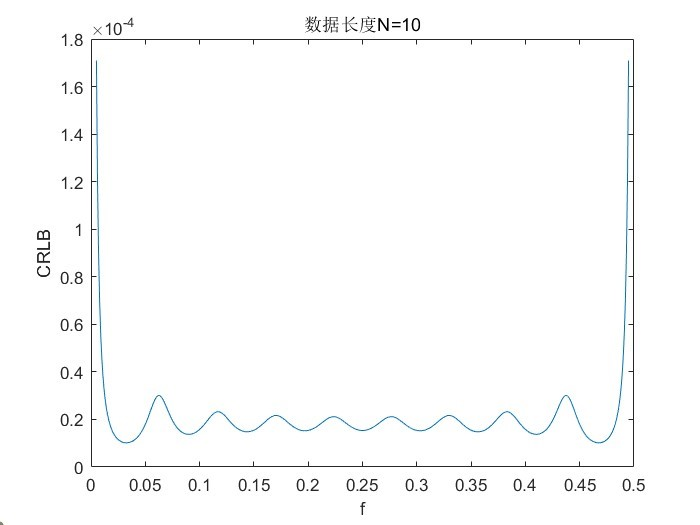
\includegraphics[scale=0.7]{fig1.jpg}
	\caption{数据长度N=10时的CRLB}
	\label{2.1}
\end{figure}

\begin{figure}[H]
	\centering
	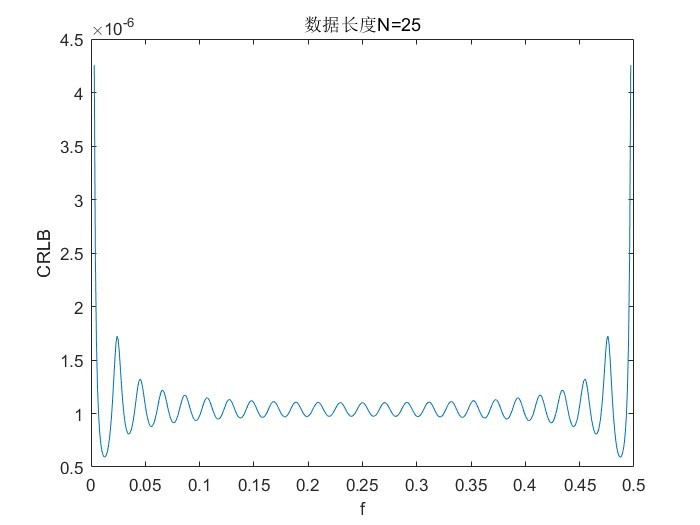
\includegraphics[scale=0.7]{fig2.jpg}
	\caption{数据长度N=25时的CRLB}
	\label{2.2}
\end{figure}

\begin{figure}[H]
	\centering
	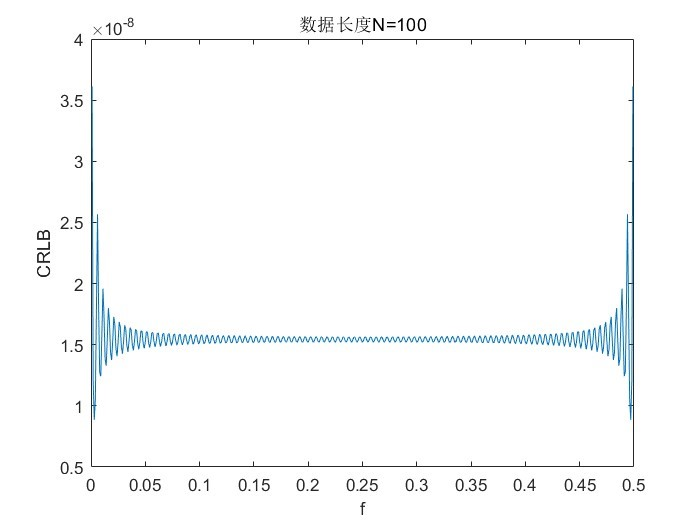
\includegraphics[scale=0.7]{fig3.jpg}
	\caption{数据长度N=100时的CRLB}
	\label{2.3}
\end{figure}

\subsection*{(3)\(A=1,f_0=0.25,f_0=0.05\)时,分别对频率参数的最大似然估计进行仿真,绘制参数估计性能随样本量、信噪比的变化曲线,
	并与克拉美-罗下限进行对比;分析验证最大似然估计的渐进性能。}

当\(A=1\)时,极大似然函数为
\begin{align*}
	p(\mathbf{x};f_0)=\frac{1}{(2\pi \sigma^2)^{\frac{N}{2}}}
	\exp\left\{-\frac{1}{2\sigma^2}\sum_{n=0}^{N-1}\left[x[n]-\cos2\pi f_0n\right]^2\right\}
\end{align*}
使得似然函数最大,等价于使指数项
\begin{align*}
	J(f_0)=\sum_{n=0}^{N-1}\left[x[n]-\cos2\pi f_0n\right]^2
\end{align*}
最小。对于集合\((0,1/2)\)内的所有\(f_0\),利用网格搜索法,可以求出\(J(f_0)\)的最小值,这时的\(f_0\)即为MLE。

\subsection*{(4)如果\(w_n\)为零均值高斯色噪声,可用如下AR模型描述
	\begin{align*}
		w_n=aw_{n-1}+e_n
	\end{align*}
	其中,\(e_n\overset{i.i.d}{\sim}N(0,\sigma_e^2),a=0.8,A=1\),试问什么情况下能够获得更准确的频率参数估计?
	试与白噪声的情况进行比较(相同的噪声方差下)。}

根据递推关系,\(w_n=aw_{n-1}+e_n\),可知
\(E(w_n)=aE(w_{n-1})\),\(var(E_n)=a^2var(E_{n-1})+\sigma_e^2\),当n足够大时,
\(E(w_n)=\frac{0}{1-a}=0\),\(var(w_n)=\frac{\sigma_e^2}{1-a^2}=\frac{\sigma_e^2}{0.36}\)。

根据中心极限定理可知,当n足够大时,\(w_n\sim\mathcal{N}(0,\frac{\sigma_e^2}{0.36})\)。
由\(e_n\)相互独立可知\(w_n\)相互独立。

问题等价于,当\(w_n\overset{i,i,d}{\sim}\mathcal{N}\left(0,\left( \frac{\sigma_e}{0.6}\right)^2\right)\)时,
求\(x_n=\cos2\pi f_0 n +w_n\)更准确的频率估计。

似然函数为
\begin{align*}
	p(\mathbf{x};f_0) & =\frac{1}{(2\pi \sigma^2)^{\frac{N}{2}}}
	\exp\left\{-\frac{1}{2\sigma^2}\sum_{n=0}^{N-1}\left[x[n]-\cos2\pi f_0n\right]^2\right\} \\
	                  & =\frac{1}{(2\pi \sigma^2)^{\frac{N}{2}}}
	\exp\left\{-\frac{1}{2\sigma^2}\left[\sum_{n=0}^{N-1}x^2[n]-
	2\sum_{n=0}^{N-1}x[n]\cos2\pi f_0 n+\sum_{n=0}^{N-1}\cos^22\pi f_0 n
	\right]\right\}                                                                          \\
	                  & =\frac{1}{(2\pi \sigma^2)^{\frac{N}{2}}}
	\exp\left[-\frac{1}{2\sigma^2}\sum_{n=0}^{N-1}x^2[n]\right]
	\exp\left\{-\frac{1}{2\sigma^2}\left[-
	2\sum_{n=0}^{N-1}x[n]\cos2\pi f_0 n+\sum_{n=0}^{N-1}\cos^22\pi f_0 n
	\right]\right\}
\end{align*}
其中,\(\sigma=\frac{\sigma_e}{0.6}\)。由于有\(\sum_{n=0}^{N-1}x[n]\cos2\pi f_0 n\)项,且其中\(f_0\)是未知的,
所以不能用Neyman-Fisher因子分解定理,即无法求出\(f_0\)的充分统计量,这时应使用最大似然估计。
要使似然函数
\begin{align*}
	p(\mathbf{x};f_0)=\frac{1}{(2\pi \sigma^2)^{\frac{N}{2}}}
	\exp\left\{-\frac{1}{2\sigma^2}\sum_{n=0}^{N-1}\left[x[n]-\cos2\pi f_0n\right]^2\right\}
\end{align*}
最大,等价于使指数项\(J(f_0)=\sum_{n=0}^{N-1}\left(x[n]-\cos2\pi f_0 n\right)^2\)最小。
对于集合\((0,1/2)\)内的所有\(f_0\),利用网格搜索法,可以求出\(J(f_0)\)的最小值,这时的\(f_0\)即为MLE。

\begin{figure}[H]
	\centering
	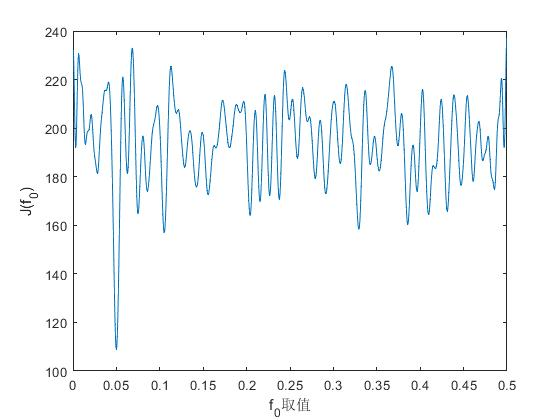
\includegraphics[scale=0.5]{fig4.jpg}
	\caption{通过J的最小值寻找\(f_0\)的MLE}
	\label{2.4}
\end{figure}

根据频率的CRLB可知
\begin{align*}
	var(\hat{f}) & \geq\frac{\sigma^2}
	{\frac{A^2}{2}\sum_{n=0}^{N-1}4\pi^2n^2(1-\cos(4\pi f_0 n))} \\
	             & =\frac{(\frac{\sigma_e}{0.6})^2}
	{\frac{A^2}{2}\sum_{n=0}^{N-1}4\pi^2n^2(1-\cos(4\pi f_0 n))}
\end{align*}
色噪声与白噪声相比,CRLB变小,估计精度变高。

\bibliography{books}
\end{document}